\documentclass{standalone}
\usepackage{tikz}
\usepackage{ctex,siunitx}
\usepackage{tkz-euclide}
\usepackage{amsmath}
\usetikzlibrary{patterns, calc}
\usetikzlibrary {decorations.pathmorphing, decorations.pathreplacing, decorations.shapes,}
\begin{document}
\small
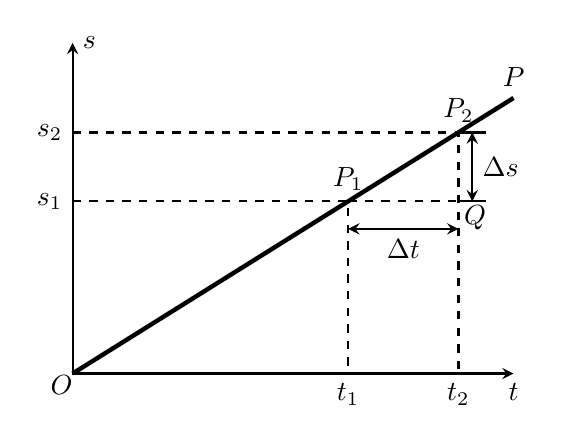
\begin{tikzpicture}[>=stealth, thick,scale=0.7]
  \draw [<->] (0,6) node[right]{$s$}--(0,0)--(8,0)node[below]{$t$};
  \node at (-.2,-.2){$O$};
  \draw[dashed] (0,5*5/8)node [left]{$s_1$}--(5,5*5/8)node [above]{$P_1$}--(5,0)node [below]{$t_1$};
  \draw[dashed] (0,7*5/8)node [left]{$s_2$}--(7,7*5/8)node [above]{$P_2$}--(7,0)node [below]{$t_2$};
  \draw[dashed] (5,5*5/8)--(7,5*5/8);
  \draw[<->] (5,5*5/8-.5)--node [below]{$\Delta t$}(7,5*5/8-.5);
  \draw[<->] (7.25, 5*5/8)--node [right]{$\Delta s$}(7.25,7*5/8);
  \draw (7, 5*5/8)--(7.5, 5*5/8); \draw (7, 7*5/8)--(7.5, 7*5/8);
  \node at (7+.3, 5*5/8-.3) {$Q$};
  \draw [ultra thick](0,0)--(8,5) node [above]{$P$};
\end{tikzpicture}
\end{document}